% This document is part of the GetRichOrDieTrying project.
% Copyright 2014 David W. Hogg (NYU).

% # to-do
% - references
% - equations
% - broader impacts
% - management plan

\documentclass[12pt]{article}
\usepackage{fancyheadings, graphicx}
\setlength{\headsep}{2ex}
%----- exact 1-in margins
% NB: headheight and headsep MUST exist and be set
\setlength{\textwidth}{6.5in}
\setlength{\textheight}{9in}
\addtolength{\textheight}{-1.0\headheight}
\addtolength{\textheight}{-1.0\headsep}
\setlength{\topmargin}{0.0in}
\setlength{\oddsidemargin}{0.0in}
\setlength{\evensidemargin}{0.0in}

%----- typeset certain kinds of words
\newcommand{\observatory}[1]{\textsl{#1}}
\newcommand{\package}[1]{\textsf{#1}}
\newcommand{\project}[1]{\textsl{#1}}
\newcommand{\an}{\package{Astrometry.net}}
\newcommand{\boss}{\project{BOSS}}
\newcommand{\des}{\project{DES}}
\newcommand{\euclid}{\observatory{Euclid}}
\newcommand{\EA}{\observatory{Exoplanet Archive}}
\newcommand{\gaia}{\observatory{Gaia}}
\newcommand{\Gaia}{\gaia}
\newcommand{\galex}{\observatory{GALEX}}
\newcommand{\Kepler}{\observatory{Kepler}}
\newcommand{\kepler}{\Kepler}
\newcommand{\lsst}{\observatory{LSST}}
\newcommand{\MAST}{\observatory{MAST}}
\newcommand{\sdss}{\observatory{SDSS}}
\newcommand{\Spitzer}{\observatory{Spitzer}}
\newcommand{\spitzer}{\Spitzer}
\newcommand{\TESS}{\observatory{TESS}}
\newcommand{\thetractor}{\package{The~Tractor}}
\newcommand{\wfirst}{\observatory{WFIRST}}
\newcommand{\latin}[1]{\textit{#1}}
\newcommand{\eg}{\latin{e.g.}}
\newcommand{\etal}{\latin{et~al.}}
\newcommand{\etc}{\latin{etc.}}
\newcommand{\ie}{\latin{i.e.}}
\newcommand{\vs}{\latin{vs.}}

%----- math shih
\newcommand{\given}{\,|\,}

%----- typeset journals
% \newcommand{\aj}{Astron.\,J.}
% \newcommand{\apj}{Astrophys.\,J.}
% \newcommand{\apjl}{Astrophys.\,J.\,Lett.}
% \newcommand{\apjs}{Astrophys.\,J.\,Supp.\,Ser.}
% \newcommand{\mnras}{Mon.\,Not.\,Roy.\,Ast.\,Soc.}
% \newcommand{\aap}{Astron.\,\&~Astrophys.}

%----- Tighten up paragraphs and lists
\setlength{\parskip}{0.0ex}
\setlength{\parindent}{0.2in}
\renewenvironment{itemize}{\begin{list}{$\bullet$}{%
  \setlength{\topsep}{0.0ex}%
  \setlength{\parsep}{0.0ex}%
  \setlength{\partopsep}{0.0ex}%
  \setlength{\itemsep}{0.0ex}%
  \setlength{\leftmargin}{1.0\parindent}}}{\end{list}}
\newcounter{actr}
\renewenvironment{enumerate}{\begin{list}{\scriptsize{\textbf{\textsf{(\arabic{actr})}}}}{%
  \usecounter{actr}%
  \setlength{\topsep}{0.0ex}%
  \setlength{\parsep}{0.0ex}%
  \setlength{\partopsep}{0.0ex}%
  \setlength{\itemsep}{0.0ex}%
  \setlength{\leftmargin}{1.0\parindent}}}{\end{list}}

%----- mess with paragraph spacing!
\makeatletter
\renewcommand\paragraph{\@startsection{paragraph}{4}{\z@}%
                                    {1ex}%
                                    {-1em}%
                                    {\normalfont\normalsize\bfseries}}
\makeatother

%----- Special Hogg list for references
  \newcommand{\hogglist}{%
    \rightmargin=0in
    \leftmargin=0.25in
    \topsep=0ex
    \partopsep=0pt
    \itemsep=0ex
    \parsep=0pt
    \itemindent=-1.0\leftmargin
    \listparindent=\leftmargin
    \settowidth{\labelsep}{~}
    \usecounter{enumi}
  }

%----- side-to-side figure macro
%------- make numbers add up to 94%
 \newlength{\figurewidth}
 \newlength{\captionwidth}
 \newcommand{\ssfigure}[3]{%
   \setlength{\figurewidth}{#2\textwidth}
   \setlength{\captionwidth}{\textwidth}
   \addtolength{\captionwidth}{-\figurewidth}
   \addtolength{\captionwidth}{-0.02\figurewidth}
   \begin{figure}[htb]%
   \begin{tabular}{cc}%
     \begin{minipage}[c]{\figurewidth}%
       \resizebox{\figurewidth}{!}{\includegraphics{#1}}%
     \end{minipage} &%
     \begin{minipage}[c]{\captionwidth}%
       \textsf{\caption[]{\footnotesize {#3}}}%
     \end{minipage}%
   \end{tabular}%
   \end{figure}}

%----- top-bottom figure macro
 \newlength{\figureheight}
 \setlength{\figureheight}{0.75\textheight}
 \newcommand{\tbfigure}[2]{%
   \begin{figure}[htp]%
   \resizebox{\textwidth}{!}{\includegraphics{#1}}%
   \textsf{\caption[]{\footnotesize {#2}}}%
   \end{figure}}

%----- deal with pdf page-size stupidity
\special{papersize=8.5in,11in}
\setlength{\pdfpageheight}{\paperheight}
\setlength{\pdfpagewidth}{\paperwidth}

% no more bad lines!
\sloppy\sloppypar

  \renewcommand{\headrulewidth}{0pt}
  \pagestyle{fancy}
  \lhead{\textsf{David W. Hogg / New Probabilistic Methods for Observational Cosmology}}
  \rhead{\textsf{\thepage}}
  \cfoot{}

\newcommand{\dd}{\mathrm{d}}
\newcommand{\data}{D}
\newcommand{\intrinsic}{\epsilon}
\newcommand{\shear}{\gamma}
\newcommand{\psf}{\psi}

\begin{document}\sloppy\sloppypar

\paragraph{Introduction}
This proposal is to improve the way we make cosmological measurements.
It is to make this improvement by building and bringing to the
community practical tools for performing probabilistic inference with
cosmological data sets.

The scale of cosmological surveys---in terms of sky area ($\pi$ to
$4\pi$ steradians), number of sources ($10^6$ to $10^9$), dynamic
range (the faintest sources can be 8~mag fainter than the brightest
sources), and heterogeneity of scientific objectives (luminosity
functions, expansion history, baryon acoustic feature)---makes them
inhospitable playgrounds for principled probabilistic inference.
Probabilistic inference (think:\ likelihood function and possibly also
Bayes) requires (in the cosmological context) generating the data, in
the sense of either being able to \emph{simulate} the data (with all
its warts) or else being able to write down a \emph{probability
  distribution in the space of the data}.
In either case, the problem is very hard:
The rawest data (pixel intensities read out by the CCD) are related to
the quantities of greatest interest only extremely indirectly, through
a model that includes not just fundamental cosmology but also the
formation of galaxies within the dark-matter density field, star
formation, intergalactic medium physics, emission and absorption and
distortions from the Earth's atmosphere, and an exceedingly complex
telescope and camera.
(We are not going to solve \emph{all} of these problems in this proposal!)

That is, it is for \emph{very good reasons} that the standard practice
of observational cosmology has a ``traditional'' feel to it:
In a typical large-scale structure survey, the standard practice is to
image the sky, create a catalog of sources, obtaining a best value for
each source's redshift (by spectroscopy or photometric redshift
estimation), compute a standard point estimate of the auto-correlation
function, and then perform cosmological inferences on that correlation
function.
This is a daisy-chain of lossy data-analysis steps; information is
lost (and noise propagation becomes approximate or impossible) each
time an intermediate point-estimate is made.
Any juncture at which we can remove one of these lossy steps, or
replace it with an information-preserving step, we will improve our
inferences, in terms of bias, and sometimes also variance.

This proposal is motivated by four observations:
\begin{enumerate}
\item
Cosmological surveys are getting bigger, and our precision demand are
getting higher.
The community has defined ``Stage-III'' and ``Stage-IV'' cosmological
projects; Stage-III is underway now, with projects like \boss and \des
and \panstarrs.
Stage-IV projects, like \lsst, \euclid, and \wfirst will be
multi-billion-source surveys that cover large fractions of the sky and
a huge part of the Hubble volume.
These projects are getting close to saturating the bounds set by the
finite volume of the Observable Universe!
We expect them to see the baryon acoustic feature at multiple redshift
slices, and detect a tiny non-Gaussianity in the initial conditions;
that is, we expect our inferences to improve as the square-root of the
sample size or na\"ive information.
Inference methods that worked in Stage-II and are being used in
Stage-III are not necessarily going to deliver completely in Stage-III
and Stage-IV:
In general, as the data get better and more numerous, inferences only
improve if the systematic errors and model errors are smaller than the
root-variance or precision of the measurements!
That is, we may be getting to a place where bigger is not better.
\item
In statistics, there is a general notion of the trade-off between bias
and variance.\footnote{For the purposes of this proposal, I am going to equate what a
statistician calls a ``bias'' with what a cosmologist calls a
``systematic error'' and what a statistician calls ``variance'' with
the inverse of what a cosmologist calls ``precision''.  I will
generally use the statistician's language.}
The current methods of cosmology make hard choices (cutting a catalog,
for example) which are equivalent (under some analysis) with making
very hard assumptions.
These assumptions are informed and informative---they con make sometimes inferences
more precise---they can sometimes reduce the variance of our inferences.
But they only make inferences more \emph{correct} inasmuch as they are
themselves correct.
We may be locking in substantial bias on our current path.
\item
In every important scientific question or data set, there are both
\emph{fundamental parameters} we care about (the cosmological
parameters, say) and \emph{nuisance parameters} we don't.
For example, we might care about the spectral index and amplitude of
the cosmological power spectrum, but we might not care about the
specific redshift of any individual galaxy in the density field.
These galaxy redshifts constitute an example of a \emph{very large}
set of nuisance parameters in any large-scale structure or
weak-lensing analysis.
Because both fundamental and nuisance parameters affect the data, both
matter; they both have to be inferred.
That is, information in the data must flow into both; the nuisances
draw information away from the fundamentals.
We will do better on the fundamentals if we don't come to firm
conclusions about the nuisances; it is better if we either never infer
them, or else marginalize them out of our final inferences about the
fundamentals.
The current standard of making a rigid catalog, point-estimating the
galaxy--galaxy or ellipticity auto-correlation function, and only
\emph{then} doing cosmological inference violates this principle.
We are measuring things we don't need to be.
That must be costing us in precision.
\item
Amazing progress has been made---in the PI's group and in the
community---in performing large, principled inferences.
We have performed astrometry and photometry on imaging without making
hard choices about the catalog limits nor requiring object detections
(Lang \etal, 2009; Brewer \etal, 2013).
There are weak and strong gravitational lensing methods that are fully
probabilistic, reconstructing cluster masses while marginalizing out
all source galaxy redshifts (\eg, Applegate \etal, 2014).
There are first attempts to marginalize out the density field in
large-scale structure (Jasche \& Wandelt, 2013; Jasche \& Lavaux, 2014).
We have performed the first inferences about the exoplanet population
that marginalize out the (very large) uncertainties on the exoplanet
radii (Foreman-Mackey \etal, 2014).
Much of the credit for this goes to applied math and computational
stats; we rely on very fast linear algebra (Ambikasaran \etal, 2014), high-end MCMC
samplers (Brewer \etal, 2013; Foreman-Mackey \etal, 2013), and distributed methods
for hierarchical probabilistic inference (Hogg \etal, 2010).
This proposal capitalizes on and leverages the PI's interdisciplinary
collaborations with applied mathematics and statistics.
\end{enumerate}

All this said, what is proposed here is going to be hard:
The dimensionality of the nuisance parameter space tends to grow with
the size of the data set.
The models of large-scale structure are fundamentally cosmological
simulations, or approximations thereto.

For example, imagine that we want to infer the auto-correlation of the
large-scale structure, but with a catalog that is based on imprecise
photometric redshifts, not precise spectroscopic redshifts.
That is, for each galaxy, there is some function $f(z)$ that expresses
either the likelihood function (probability of the data given the
redshift) or the posterior pdf (probability of the redshift given the
data).
How would we use such information in correlation-function inference?
Current practice---when there are rigid redshift estimates rather than
redshift probability functions---is to count pairs of galaxies and
build the correlation function estimate out of histograms of pair
counts from the data and from ``random'' (unclustered; Poisson)
catalogs with a similar selection function.
With the redshift functions $f(z)$ what to do?
You can resample the data from $f(z)$ and make correlation-function
estimates from the resampled data.
This is \emph{completely wrong}.
It constitutes, in effect, re-convolving the data with the
uncertainty; reducing the precision of inferences and substantially
biasing the results.

The right thing to do is draw samples of the density field \emph{and}
the true redshifts, where the weight of such samples in the answer is
in proportion to the likelihood---the probability that the density
field and the true redshifts can generate the positional data.
This requires an ability to (within the data-analysis iteration loop)
draw density fields.
It also requires a jettison of the whole idea of the point estimate
(Landy--Szalay estimator or whatever) of the two-point function; there
is no use of such an estimator within this inference in which the
redshift inferences are being penalized by their consistency with the
density field.
That alone appears intractable at the present day (but see below), and
this is just one of many problems faced by a principled probabilistic
reasoner in cosmology.

This proposal, in some sense, is to develop the \emph{theory} of
experimental cosmology, plus tools to execute some approximation
to that, tractably.

One side note worth making here is that there is a huge literature
already on the theory of cosmological observables.
There is work on making more and more precise predictions for the
non-linearities induced by gravity, the distortions caused by our
working in redshift (rather than pure position) space, the shape of
the baryon acoustic feature as a function of redshift, and the
statistics of the shapes of galaxies and covariances in those induced
by galaxy--galaxy interactions (so many good theory papers that it
would be impossible to fairly cite this literature, and also beside
the point).
This work is getting ever more sophisticated and remarkable, as the
practitioners of observational cosmology demand higher and higher
precision predictions to match the higher and higher precision of the
data.
Indeed, this whole literature and community stands as a great example
of how mature science ought to work:
Interactions between large observational efforts and large theoretical
efforts, every step improving our ability to refine and rule out
models.

The projects proposed in this proposal are \emph{perfectly
  complementary} to other theory work in cosmology.
Indeed, any inference performed with the toolsets I propose will
simultaneously make use of the best practical predictions emerging
from the body of cosmology theory.
The projects proposed in this proposal are also \emph{perfectly apt},
in some form, for \emph{any} cosmological data set.
That is, what is proposed here leverages all cosmology theory and the
capabilities of all new observational projects to make cosmological
measurements less biased and more precise.

\paragraph{Why this PI?}

If you are convinced that precise cosmological measureents are
important, and if you are convinced that data sets are getting more
precise, then it is hard to deny that we should be looking at whether
our measurement precision is limited by our inference or measurement
tools.
The hard questions are: Who should do this, and is there any chance it
is even possible, anyway?
Although the projects proposed (below) are ambitious, the PI's group
has a range of theoretical, technical, and technological successes
that make it the ideal to work towards the proposed goals:
\begin{itemize}
\item
In exoplanet and astrometric research contexts, we have developed valuable new Markov
Chain Monte Carlo sampling technologies, including affine-invariant
samplers (Hou \etal, 2012; Foreman-Mackey \etal, 2013), nested
samplers (Hou \etal, 2014), reversible-jump nested samplers (Brewer
\etal, 2013), and elliptical slice samplers (Foreman-Mackey \etal,
2014).
\item
We have developed novel methods (based on importance sampling) for
performing hierarchical probabilistic inferences in problems where
data sets are large.  These methods have permitted us to perform the
inferences ``in the data center'' rather than in a single core (Hogg
\etal, 2010; Foreman-Mackey \etal, 2014).
\item
In spacecraft and survey self-calibration projects, we have built
data-driven models of instrument throughputs and sensitivity with
hundreds of millions to billions of parameters (Padmanabhan \etal,
2008; Holmes \etal, 2012) and we now have a model of the
\kepler\ focal plane with (literally) more than $10^9$ parameters per
target star!  These models are incredibly flexible but the methods are
designed so that they can \emph{only} fit out variability in the data
that does not project onto the astrophysical signals of interest.
\item
We have built systems to perform pixel-level image modeling to create
probabilistic catalogs, probabilistic photometric information,
probabilistic source separation and deblending, and prior-influenced
photometry in astronomical imaging.  There is a huge project called
\thetractor\ that we have started, and it is bearing fruit in a
massive re-analysis of the \observatory{WISE} data (Lang \etal, 2014) and weak
lensing (next up).
\item
In cosmological weak lensing, we have built the first-ever shear-field
measurement code that delivers likelihood about the shear field based
only on the pixel values from the telescope, marginalizing out beliefs
about any individual galaxy (Schneider \etal, 2014).  We entered the
\project{GREAT3} weak lensing challenge with this code, which can
perform the sampling and marginalization at scale.
\item
Gaussian process regression and density estimation require---when you
want to infer the hyperparameters too---not just fast, large matrix
factorizations and solves, but also fast determinant calculations.
When you want the hyperparameters to represent some physical reality
(like the Universe), it is not possible to keep these matrices sparse.
We have the fastest method and code in the world for
machine-precision, fast, dense matrix operations (Ambikasaran, 2014).
\item
We have performed Gaussian-process-controlled inference in a context
in which the data are noisy in all dimensions, including the
``features'' used for the Gaussian process (Foreman-Mackey \etal,
2014).  This is a classically ``hard'' problem in machine learning,
but we now have technology that seems to work for small problems and
there is hope for scaling up.
\end{itemize}

In addition to all these technical achievements, all of which are
relevant to what follows, the PI has a positive and valued pedagogical
role in the astrophysics community.
He is invited to participate as teacher or co-organizer in roughly
four astronomical statistics and data-analysis workshops and schools
each year (most recently at SAMSI, CMU, UW Seattle, and ESAC in
Madrid); about half of his dozen research seminars per year focus on
data analysis and statistical inference (most recently a plenary talk
at the American Astronomical Society, and Toronto, Princeton, and MPIA
in Heidelberg).
He is known for putting pedagogical texts on the arXiv, most notably
on cosmological distance measures (Hogg, 1999) and on fitting data
with simple models (Hogg \etal, 2010b).
These are not strictly relevant to the technical goals of this proposal,
but they will increase the potential for \emph{broader impact} of this work, and
help make sure the methods and tools get used as widely as possible.

\paragraph{\package{Toolset 1}: Density-field inference and marginalization}

The standard estimator for the auto-correlation function of galaxies
is a point estimator that makes two critical assumptions:
It assumes that the galaxy positions are perfectly known, and that the
density field is a Gaussian random field, with only a mean value and
variance structure.
On the latter point---Gaussianity---the assumption came in by way of
\emph{efficiency}; the estimator only saturates the Cram\'er--Rao
bound if the density field is a Gaussian random field.

If all of cosmology is built on these hard (and known wrong)
assumptions, we can only do better by relaxing them.
We can relax them both if we can make practical ways of generating the
galaxy density field---or mass density field---simultaneously
constrained by the observed galaxy positions \emph{and} the
correlation function.
That is, we need to be able to build a simultaneous probabilistic
model of the three-dimensional data field \emph{and} all of the true
redshifts, constrained by the data (the galaxy positions and the weak
redhift information).

Schematically, we could write down the plan like this:
\begin{equation}
p(d\given \Omega) = \int p(d\given z)\,p(z\given \rho)\,p(\rho\given \xi)\,p(\xi\given \Omega)\,\dd z\,\dd\rho\,\dd\xi
\end{equation}
where $d$ represents all the data, $z$ represents all the galaxy
positional information, $\rho$ represents the density field, $\xi$
represents the correlation function or power spectrum of the density
field, and $\Omega$ represents the cosmological parameters.
\package{Toolset~1} aims to make the functions $p(z\given\rho)$ and
$p(\rho\given\xi)$ tractable to sample from, infer, and integrate out.
Note that this equation (above) is only intended to be schematic;
there are a lot of details, since $d$, $z$, $\rho$ and so on are very
complex, heterogenous objects.  This equation is also an example of a
hierarchical model: $\xi$, for example, only affects $z$ by the fact
that it generates $\rho$ which in turn generates $z$.  That
hierarchical structure is exploited in our sampling and integration
strategies.

This big probabilistic model is a bit scary.
There is one regime in which this can be feasible:
Using a Gaussian Process (Rasmussen \& Williams, 2006), for which we currently have
the fastest code in the world (Ambikasaran \etal, 2014), we can draw density fields
constrained by data (draw from $p(z\given\rho)$) for any true-redshift realization, in the case
when the density field is indeed Gaussian!
That is, the project proposed here is easier at larger scales (where
the density is closer to Gaussian) and harder at smaller scales (where
fully cosomological simulations become more important).

In addition, where the density field is weakly non-linear, there is a close
relationship between the density field and the Gaussian initial
conditions, so it is possible to draw Gaussian initial ``latent''
fields and then distort them according to second-order perturbation
theory to make realistic, weakly non-Gaussian density fields.
We believe that this project is feasible; there are examples in
the machine-learning literature of full inference in a model of a
field that is a distortion of a Gaussian random field, and then
sampled by points (galaxies, in our case).

One challenge of this approach is that out-of-the-box Gaussian Process
packages do not permit specification of an \emph{arbitrary}
correlation function (covariance function or kernel function) for the
latent field.
Here, one of the objectives is to \emph{determine} the correlation
function, and indeed \emph{marginalize out} the density field (and all
other nuisances).
This requires a method for specifying arbitrary correlation functions.
With Mike O'Neil (NYU Math) and Jon Wilkening (Berkeley Math), we have
developed a fully general expansion for positive-definite covariance
functions that correspond to free functions for the correlation
function.
This expansion---plus an ability to take large matrix determinants
(which we have; Ambikasaran \etal, 2014)---will permit simultaneous inference of the
latent field controlling the density, the correlation function, and
any aspects of galaxy position (say redshifts) that are uncertain.
Since we will sample in all dimensions with MCMC (or, realistically, a
Gibbs or slice-sampling version of MCMC), it will be possible to
deliver posterior samples for the correlation function \emph{fully
  marginalized} over density and galaxy-position realizations.
This full set of capabilities comprise \package{Toolset~1}.

There is some prior work in this area, most notably by Jasche \&
Wandelt (2013) and Jasche \& Lavaux (2014).
Our differences with them are first, our very fast linear algebra, the
fastest in the world, second, our methods for expanding the
correlation function in real space, and third, our commitment to build
and release useful tools.
That said, the success of Jasche and collaborators is one of the
things that has inspired us to propose building these toolsets.

We propose to develop and execute a method of this kind to perform
large-scale structure inference at intermediate regimes (few Mpc and
larger).
We will test this method on the Stage-III \boss\ galaxy data, and show
that we confirm or improve on results obtained by the standard
methods.
This real-data test will both demonstrate the methods functionally,
and make us into not just the builder of the toolset but also the
\emph{customer} for the toolset.
It is our experience that tools are much better built when the
customer is involved.

It is possible that our work on the \boss\ data will create
different answers (because bias has been reduced) or more precise
answers (because the model is more appropriate) than have been found
previously.
Obviously, if this is the case, we will work to understand the
differences and from where they emerge.

In terms of outputs from this proposal, in addition to the code for
\package{Toolset~1}, we will also publish a theory and method-oriented
paper, and also a data and results paper from the \boss\ experiment.
We will release the toolset as documented, MIT-licensed, open-source
code.

\package{Toolset~1} will make fewer assumptions than the standard
methods for cosmological inference.
In particular, it will estimate the correlation function with an
implicit generative model that is more correct than that underlying
the Landy--Szalay estimator.
It ought, therefore, to provide less biased cosmological results.
However, it will not necessarily provide lower variance results (more
precise results).
This is because the method is \emph{also} more flexible.

The density estimation and correlation inference made possible by
\package{Toolset~1} is very general; it could be applied to other
kinds of density fields, such as the two-dimensional projected
mass-density field observed with weak lensing, and the neutral-gas
density field absorbed through quasar absorption lines.
Inasmuch as time permits, such inferences represent enhanced goals
that could be pursued by the project personnel.

\paragraph{\package{Toolset 2}: Using and improving probabilistic redshift information}

For the faintest sources in the Stage-IV projects (and even, say, the
Stage-II \sdss\ imaging), there is no accurate redshift information.
Indeed, there can't be:
We can never take spectroscopic data as faint as we can do imaging,
and photometric redshifts are not just somewhat imprecise, they are
difficult (or perhaps impossible) to calibrate or test where no
spectroscopy is available.
In addition, we want to be able to use in large-scale structure and
cosmology projects sources that did not get spectroscopy for other
reasons, or where spectroscopy is ambiguous or low in signal-to-noise.
In the brave future of Stage-IV projects, we expect this to be the
vast majority of sources of interest.

Facing this reality, many projects---but in particular \lsst---are
planning on creating and delivering redshift probability products,
which describe either the redshift likelihood function for each source
or else the redshift posterior under simple priors.\footnote{It turns
  out that we \emph{always} want the likelihood function, and
  \emph{never} want the posterior pdf for the redshift.  The reasons
  for this are technical; they relate to the marginalizations that are
  required.  No more will be said about this, but the PI has polemics
  available (``Telescopes don't make catalogs'', Hogg \& Lang 2011).}
The question is:  How should we use these probabilistic outputs?
Most proposed (and some actual) uses of these have turned out to be
misguided, in the sense that they are not expected to improve the
biases in resulting inferences.
That is, there are no \emph{inexpensive} uses of probabilistic
redshift information that improve inferences; all the inexpensive
ideas make things \emph{worse}.

For the purposes of this proposal, two general areas where
probabilistic redshift information might be used will be discussed:
the inference of galaxy luminosity functions (and their evolution) and
the inference of the large-scale structure correlation function.
In each case, it is tempting for an investigator, faced with
probabilistic redshift information, to resample the galaxy population,
drawing for each galaxy randomly from its redshift probability
distrubution.
Then the investigator could perform inference for each such draw and
take the distribution over results to be a propagation of the redshift
noise into the results.
This kind of approach has been performed multiple times in the
cosmological literature.

It turns out that all methods of this kind are incorrect:
They treat the probabilistic redshift functions as applying to the
data---as being tools for distorting the data.
They are not!
Distorting the data is never appropriate, and in the cases of interest
here will enworsen any results.
The redshift functions apply to the model (the latent, true redshifts); they are tools
for distorting the \emph{predictions} to make them match the data.
That is, the probabilistic information about redshift must be used in
the data-generating model.
They must be used as part of a data simulation or a likelihood
function (probability in the data space).
The cool bonus thing is that when they are used in this way---as part
of a generative model---not only do they improve inferences, the
inference will \emph{also} return improved redshift estimates.  That
is, the inference gets better \emph{and} the model provides
information back to the redshifts.
This is the magic of hierarchical modeling.

In the case of luminosity-function inference,
the idea is that any parameterized model of the luminosity function
(even a very general model that is, say, a mixture of Gaussians or a
step function with hundreds of steps) is a model of how galaxy
luminosities and redshifts are generated (by the fundamental or
effective model).
The model for how the data are generated from those luminosities
involves the redshift likelihoods; they take true galaxy redshifts and
luminosities (and other spectral properties) and give back a
probability for the data.
The individual-object redshift likelihood functions are tools that
take a model that can generate true redshifts and convolve that model
into one that generates the \emph{data}.
Then, within that model, all the galaxy true redshifts and
luminosities are model parameters (possibly nuisance parameters) to be
inferred along with the luminosity-function parameters.
The redshifts and luminosities can be marginalized out to provide good
luminosity-function estimates,
or the luminosity-function parameters and luminosities can be marginalized
out to provide better redshift estimates.
\package{Toolset~2} will perform this hierarchical inference.

Schematically, here, we could write:
\begin{eqnarray}
p(d\given \Phi) &=& \int p(d\given L, z)\,p(L, z\given \Phi)\,\dd L\,\dd z \\
p(d\given z) &=& \int p(d\given L, z)\,p(L, z\given \Phi)\,\dd L\,\dd\Phi
\end{eqnarray}
where $d$ represents all the data, $L, z$ represents all the galaxy
luminosity and redshift information, and $\Phi$ represents the redshift-evolving luminosity function.
In the first case we are inferring the luminosity function, integrating out
the luminosities and redshifts.
In the second case we are getting better redshift estimates, integrating out
everything else.
Again, there are a lot of details, since $d$, $L$, $z$, and $\Phi$ and so on are very
complex, heterogenous objects.

In the literature, some have ``propagated'' the redshift uncertainty
into the luminosity uncertainty, and measured the luminosity function
using less precise but more conservative luminosity uncertainties.
While this approach is more conservative and less biased than ignoring
the redshift uncertainty, it does not deliver the precision of a
hierarchical inference.
That's because it does not use the learning about the luminosity
function to simultaneously improve the redshift estimation and vice
versa.
It doesn't capture all of the information available from our understanding
that the true redshifts are ``generated'' by the model.
We have demonstrated this (in exoplanet contexts) in several projects
now (Hogg \etal, 2010; Foreman-Mackey \etal, 2014).
Again, \package{Toolset~2} will give us and the community these powers.

In the case of correlation-function inference, the story is very much
the same, only harder to execute:
Now the model has correlation-function parameters, which in turn act
like priors on the a latent ``true'' density field, and then the
galaxies are samples of either that field or else a ``true'' galaxy
field from which galaxies are generated.
(This only works for scales $>$Mpc, where galaxy generation can be
seen as a local, independent process.)
Now each galaxy ``true'' redshift can be informed both by the likelihood
function $f(z)$ and also the current inferences about the density field
that are themselves informed by the correlation function.

Schematically, this is:
\begin{eqnarray}
p(d\given \xi) &=& \int p(d\given z)\,p(z\given \rho)\,p(\rho\given \xi)\,\dd z\,\dd\rho \\
p(d\given z) &=& \int p(d\given z)\,p(z\given \rho)\,p(\rho\given \xi)\,\dd\rho\,\dd\xi
\end{eqnarray}
where once again, $d$ represents all the data, $z$ represents all the galaxy
positional information, $\rho$ represents the density field, and $\xi$
represents the correlation function or power spectrum of the density
field.  Again, the latter uses the density field to improve the redshift estimates.
That sounds like the tail wagging the dog, but it might be immensely powerful.

This whole chain of reasoning comprises a hierarchical inference that
makes use of \package{Toolset~1} for density-field inference, and
also work we have done in exoplanet contexts (Foreman-Mackey \etal, 2014) to infer a
Gaussian process in the face of data points with noisy \emph{locations}.
This requires, for efficiency, specialized samplers, one
of which we will release along with everything else in
\package{Toolset~2}.

We will use \package{Toolset~2} to measure the luminous red galaxy
(LRG) luminosity function and its evolution, and also the clustering
of luminous red galaxies on intermediate and large scales, in the
\sdss\ imaging data.
One goal is to reproduce what is known about the LRG luminosity
function, another the correlation function, including the baryon
acoustic feature (Eisenstein \etal, 2005).
For the LRG redshifts, we will use not the spectroscopic redshifts but
instead the photometric redshifts, to make sure that $f(z)$ is
non-trivial for all sources.
Because we will be re-inferring for a known population but with worse
data, we---in some sense---know the truth, or what we must get in the
best possible case.
That makes this \sdss\ analysis a true functional test of
\package{Toolset~2}; this is important, because it is such a radical
departure from the standard methodologies.

In the test of \package{Toolset~2} with \sdss\ we can not just try to
reproduce the cosmological quantities, but also to obtain better
posterior beliefs about the redshifts.
This will be another output of the hierarchical model.
Again, since we know the spectroscopic redshifts, we can test these
posterior inferences in a very strong way.

The deliverables of this part of the proposal will be the
\package{Toolset~2} code, and two papers, one that is theory and
method oriented, and another that reports the results of the testing
and inferences on the \sdss\ imaging data.
Again, we will try to understand in these papers the quantitative
differences we get with the (now famous) results of \sdss.

\paragraph{\package{Toolset 3}: Creating and using probabilistic shape and PSF information}

Cosmic shear, small distortion of the images of distant
galaxies by large-scale structure in the universe,
is a major probe of cosmolgy. Measurement of the cosmological
weak lensing signal provides extremely powerful probe of the
evolution of dark energy, since the shear signal depends on
both the growth of structure, and the distance-redshift relation.
In this document we present tractable probabilistic methods that
make less constraining assumption about the flow of information
from the data to the cosmological parameters, and help us fully exploit
the potential of weak lensing in  constraining cosmology using the
imaging data from wide field surveys.

PSF estimation for weak lensing:
Extracting the cosmic shear from galaxy images is one of the most challenging tasks in astronomical
data analysis. Shear signal induced by lensing on the images of background galaxies
is coherent but much smaller than the typical 
ellipticities of those galaxies. Moreover, the image of lensed galaxies is convolved with 
an unknown spatially varying kernel, the Point spread function, whose typical
anisotropy is greater than the cosmic shear itself.
 
Effectively, we have 
noisy estimates of the PSF at the positions of stars. We need to use these estimates to infer the
underlying two dimenstional pattern of the PSF. The spatial variation at large angular scales is 
generally smooth and can be well-modeled by the high signal-to-noise stars. However, both atmospheric
turbulance and telescope optics, introduce PSF that varys on scales smaller than the distance
distance between the bright stars. 

Inaccurate estimation of the PSF at the positions of galaxies will lead to bias in shear estimates,
which will propagate into the dark energy constraints if not accounted for. In order to
tackle this issue, we propose to infer the propability distribution function over the PSF
at the positions of galaxies, so that we can marginalize over the PSF instead of treating it 
as a rigid object.

This probability distribution function (a) needs to be flexible enough to capture the complicated 
features of the shape of the PSF as well as its spatial variation, (b) needs to propagate uncertainties
from the pixel level to the PSF, and (c) needs to be easy to evaluate and easy to sample from. By 
projecting the images of stars into lower dimensional KL basis, and imposing Gaussian Process priors 
over each direction of the KL basis we satisfy all the mentioned requirements. This model successfully propagates
the uncertainties in the form of a posterior PDF over PSFs; 
that is, it returns probabilistic information about the PSF at the positions of galaxies. At each
position of the astronomical image, this posterior PDF has a simple form of a Gaussian.

We also examine the performance of this method on estimation of the PSF for simulations 
of \lsst. First, we identify the bright stars on the image and then we randomly divid
them to training set and validation sets of equal size. After learning the KL basis and 
hyper parameters of the Gaussian Process model in the training set, we infer the posterior 
PDF of PSF at the position of stars in the validation set. Figure [\ref{1}] shows a star
in the validation set, and three different draws from the posterior PDF of PSF at that position.

probabilistic inference of shear:
Typically, after measuring the shapes
of a large ensemble of galaxies in a way that
the effect of PSF is elliminated, ellipticities
of these galaxies are averaged together in order to
find a point estimator of the shear.
The methods based on ensemble averaging make strong assumption
about the probability distribution of the intrinsic shape parameters,
and are able to deliver unbiased estimate of shear only if we
have access to unbiased measurements of individual galaxy
ellipticites. 

Our aim is to deliver a fully probabilistic approach for estimation of shear.
We want to write down a likelihood function $p(\data_n\given\shear)$, where $\{\data_n\}$
represents the set of galaxy images. In order to do so, we need to marginalize over the
nuisance parameters that we do not care about. This set of nuisance paramters includes 
shape parameters (e.g., ellipticities), non-shape parameters (e.g., flux, centroid, etc.)
of galaxies, and also the PSF

\begin{eqnarray}
p(\data_n\given\shear)
  &=& \int p(\data_n\given\intrinsic_n , \omega_{n}, \psf , \shear)
  \,p(\intrinsic_n, \omega_{n})\,p(\psf)\,\dd\intrinsic_n\,\dd\omega_n\,\dd\psf
  \quad ,
\label{integral}
\end{eqnarray}
where $\{\intrinsic\}$ ($\{\omega_{n}\}$) represents the set of shape
(non-shape) parameters.

Schematically, equation (\ref{integral}) can be shown by the probabilistic
graphical model (PGM) in Figure[\ref{2}]. Therefore, in this model we need
a prior PDF over intrinsic (unlensed, PSF deconvolved) parameters of galaxies.
This can be done by (a) finding a deep subset (containing a large number of high
signal-to-noise galaxies) of the data, (b) finding the maximum-likelihood estimates
of parameters of those galaxies, (c) and fitting an empirical prior to those parameters. 

Importance sampling ........

multi-exposure data:
The imaging data from the upcoming WL surveys will consists of several
short exposures of each individual galaxy. Stacking has been widely used
as a method to combine information from multiple exposures. 
Although stacking is able to deliver high signal-to-noise images, it distroys a
huge amount of information regarding the spatial variation of
the PSF, and it involves image transformation that could lead to correlated noise
in the final product and distortion of the PSF.

An important advantage of our model is that it can be easily extended
to making inference of shear from multi-exposure data. The graphical model 
regarding corresponding to application of our probabilistic inference to
multi-exposure data is shown in Figure[\ref{3}].

\paragraph{Broader impacts}

As mentioned above, the PI has been an active author of methods,
software, and pedagogical documents for the astrophysics and cosmology
communities.
These documents are aimed at undergraduate physics majors, graduate
students, and professional researchers.
He has also been active in professional education from undergraduate
through to research professional, influencing a large part of the
community.
The tools he has released have had an impact in a huge set of domains,
and made it possible for different groups to think differently about
their data and experiments.

The PI is also a member and an administrator of the NYU Center for
Data Science.
This interdisciplinary (and inter-school) initiative at NYU is hiring
faculty in joint appointments, starting a PhD program between the
methods and the science domains, running a masters program, and
operating events to educate all levels of the NYU and NYC communities
about data and inferences from data.
This has given the PI many opportunities to translate methodological
ideas for domain scientists, especially early-career and junior
members of the community.
It has also given great opportunities to advertise astronomical
research and data sets to the methods communities; the latter has led
to many new projects in computer science, applied mathematics, and
statistics.
These activities are having an effect on research and education across
the university and in the community of research universities, through
curriculum development, career-path analysis, and new roles for
scientists, engineers, and developers in science projects and the
academy.

Examples of the PI's success in interdisciplinary work are given
above; they include co-authored publications with faculty in the three
classes of methods departments---Mathematics, Statistics, and Computer
Science---and tools with high uptake.

In addition to all this, the PI has influential arXiv-only documents
(\project{Data Analysis Recipes}) with pedagogical content, and as
part of this proposal proposes to write three more,
\begin{enumerate}
\item
a \project{Data Analysis Recipes} on model selection, discussing
traditional methods related to $chi^2$ improvement, engineering
methods of cross-validation, pure Bayesian methods, and practical
decision theory,
\item
a \project{Data Analysis Recipes} on MCMC sampling, discussing the
basic method, initialization, burn-in, tuning, convergence analysis,
and trouble-shooting,
\item
and a \project{Data Analysis Recipes} on Gaussian processes,
discussing non-parametrics, regression, inference, and sampling, noise
modeling, linear algebra, noisy features, and high-dimensional feature
(ambient) spaces.
\end{enumerate}
Each of these techniques or issues is either highly used in astronomy
or growing fast, and many students are encountering similar issues.
Perhaps more importantly, these kinds of subjects are becoming a part
of the physics and astronomy undergraduate curriculum.
If we can move the curriculum in this direction, that would be a very
satisfying broader impact of the proposed work.

One of the ways that the PI is influential (on the youth, anyway) is
by participating in Hack Days and other informal-education events (see
above and below for more details).  This will continue and serve to
create and amplify these broader impacts.

\paragraph{Prior NSF support}

The PI has been supported by a Cyber-Enabled Discovery Type I Grant
(IIS-1124794; Hogg, PI), \textit{A Unified Probabilistic Model of
  Astronomical Imaging}.
This grant has supported work by NYU graduate students Daniel
Foreman-Mackey and Dilip Krishnan, and NYU postdoctoral scholar Ross
Fadely.
Foreman-Mackey is finishing his PhD at NYU this Spring, and Krishnan
is now a postdoctoral scholar in computer science at MIT.
The grant was explicitly inter-disciplinary between computer vision
and astrophysics.

This grant has supported 13 refereed publications.
In the category of \textbf{Intellectual Merit},
research highlights from this grant include the most highly used MCMC
sampler in the astrophysics community (Foreman-Mackey \etal, 2013)
with more than 200 citations in one year, the
first-ever near-infrared spectroscopy of exoplanets (Oppenheimer \etal, 2013;
Fergus \etal, 2014), and a likelihood function for the exoplanet population
in terms of (or conditioned on) the pixel values telemetered down by
the NASA \kepler\ Satellite (Foreman-Mackey \etal, 2014).

In the category of \textbf{Broader Impacts},
in addition to the publications, this grant has supported the creation of
many open-source code-bases.
The most notable is that of \package{emcee}, mentioned above, which is
one of the top physics-related github repositories in the world.
But in addition to this, the personnel on this grant have opened and
developed in dozens of other repositories, with code under open
licenses (usually MIT).

Also along the broader-impacts line, Foreman-Mackey and the PI have
been operating Hack Days at the American Astronomical Society
meetings, at the dotastronomy meetings, and at AstroData Hack Week,
which will be called AstroHackWeek going forward.
The PI and Foreman-Mackey have been invited to give talks and
participate in summer schools (including the AstroStatistics school at
Penn State and a European equivalent in the Canary Islands) on
pedagogical subjects related to MCMC sampling, Gaussian Processes,
hierarchical inference, and data analysis.
The combination of computer vision and astronomy supported by the
grant is gaining traction in the astronomical community at large, and
astronomical data sets and problems are becoming more visible in the
computer vision community.

The PI has been supported in the past by other NSF grants, including
NSF Astronomy and Astrophysics Research Grant (AST-0908357; Hogg, PI),
\textit{Dynamical models from kinematic data:\ The Milky Way Disk and Halo,}
NSF Information Technology Research Grant (AST-0428465; Hogg, PI),
\textit{Automated Astrometry for Time-Domain and Distributed
Astrophysics,} and
NSF Group Grant (PHY-0101738; Farrar, PI), \textit{Theoretical
Particle Physics, Astrophysics and Cosmology.}
These grants supported postdocs and graduate students and many dozens
of refereed publications.

In addition to this NSF support, the PI also has some NASA support and
is involved in the administration of the Moore--Sloan Data Science
Environment at NYU.
Although the latter grant is a large award, it does not directly
support the research of this PI.
It supports broad data-science programs at NYU which operate
independently of the PI's group or research.

\paragraph{Project management and products}

This project is very lean; it is comprises just a PI and two
students, one of them part-time.
The rough scheduling would be to work on \package{Toolset~1} and
\package{Toolset~3} in year one, \package{Toolset~2} in year two, and
finish all paper-writing and documentation of code in year three.
The ordering of toolsets is based on the current level of shovel-readiness
in the PIs group as of today.
It would be nice to write the theory and method papers prior to the
real-data papers, but this is probably not realistic; they will
probably have to be written together, given the interplay between
functional testing and theory in these projects.
Another way to put it: The approximations and methods will be strongly
driven by what really works with real data.

The toolsets will be released publicly under the MIT open-source
license using the platform \project{github} or equivalent.
We also expect to work in a generally open mode, so that all of our
work can be seen and inspected as it is underway.
We have had great success in this mode and it has brought a lot of
expertise and visibility to the group and our projects.

The PI will produce, with student help and co-authorship as
appropriate, \project{Data Analysis Recipes} papers, one per year, on
the topics mentioned above.

At two meetings per year, the American Astronomical Society winter
meeting, and the new, annual \project{AstroHackWeek} meeting
co-organized by NYU, University of Washington, and UC Berkeley, we
will operate hack sessions.  These will be organized by the PI, but
with expected participation, both in hacking and in leading and
teaching, by the students.
These hack sessions at these meetings have already been established by
the PI, so these involve no new development or risk; indeed they are
already highly successful operations.

\clearpage

\begin{figure}[!htb]
\minipage{.8\textwidth}
  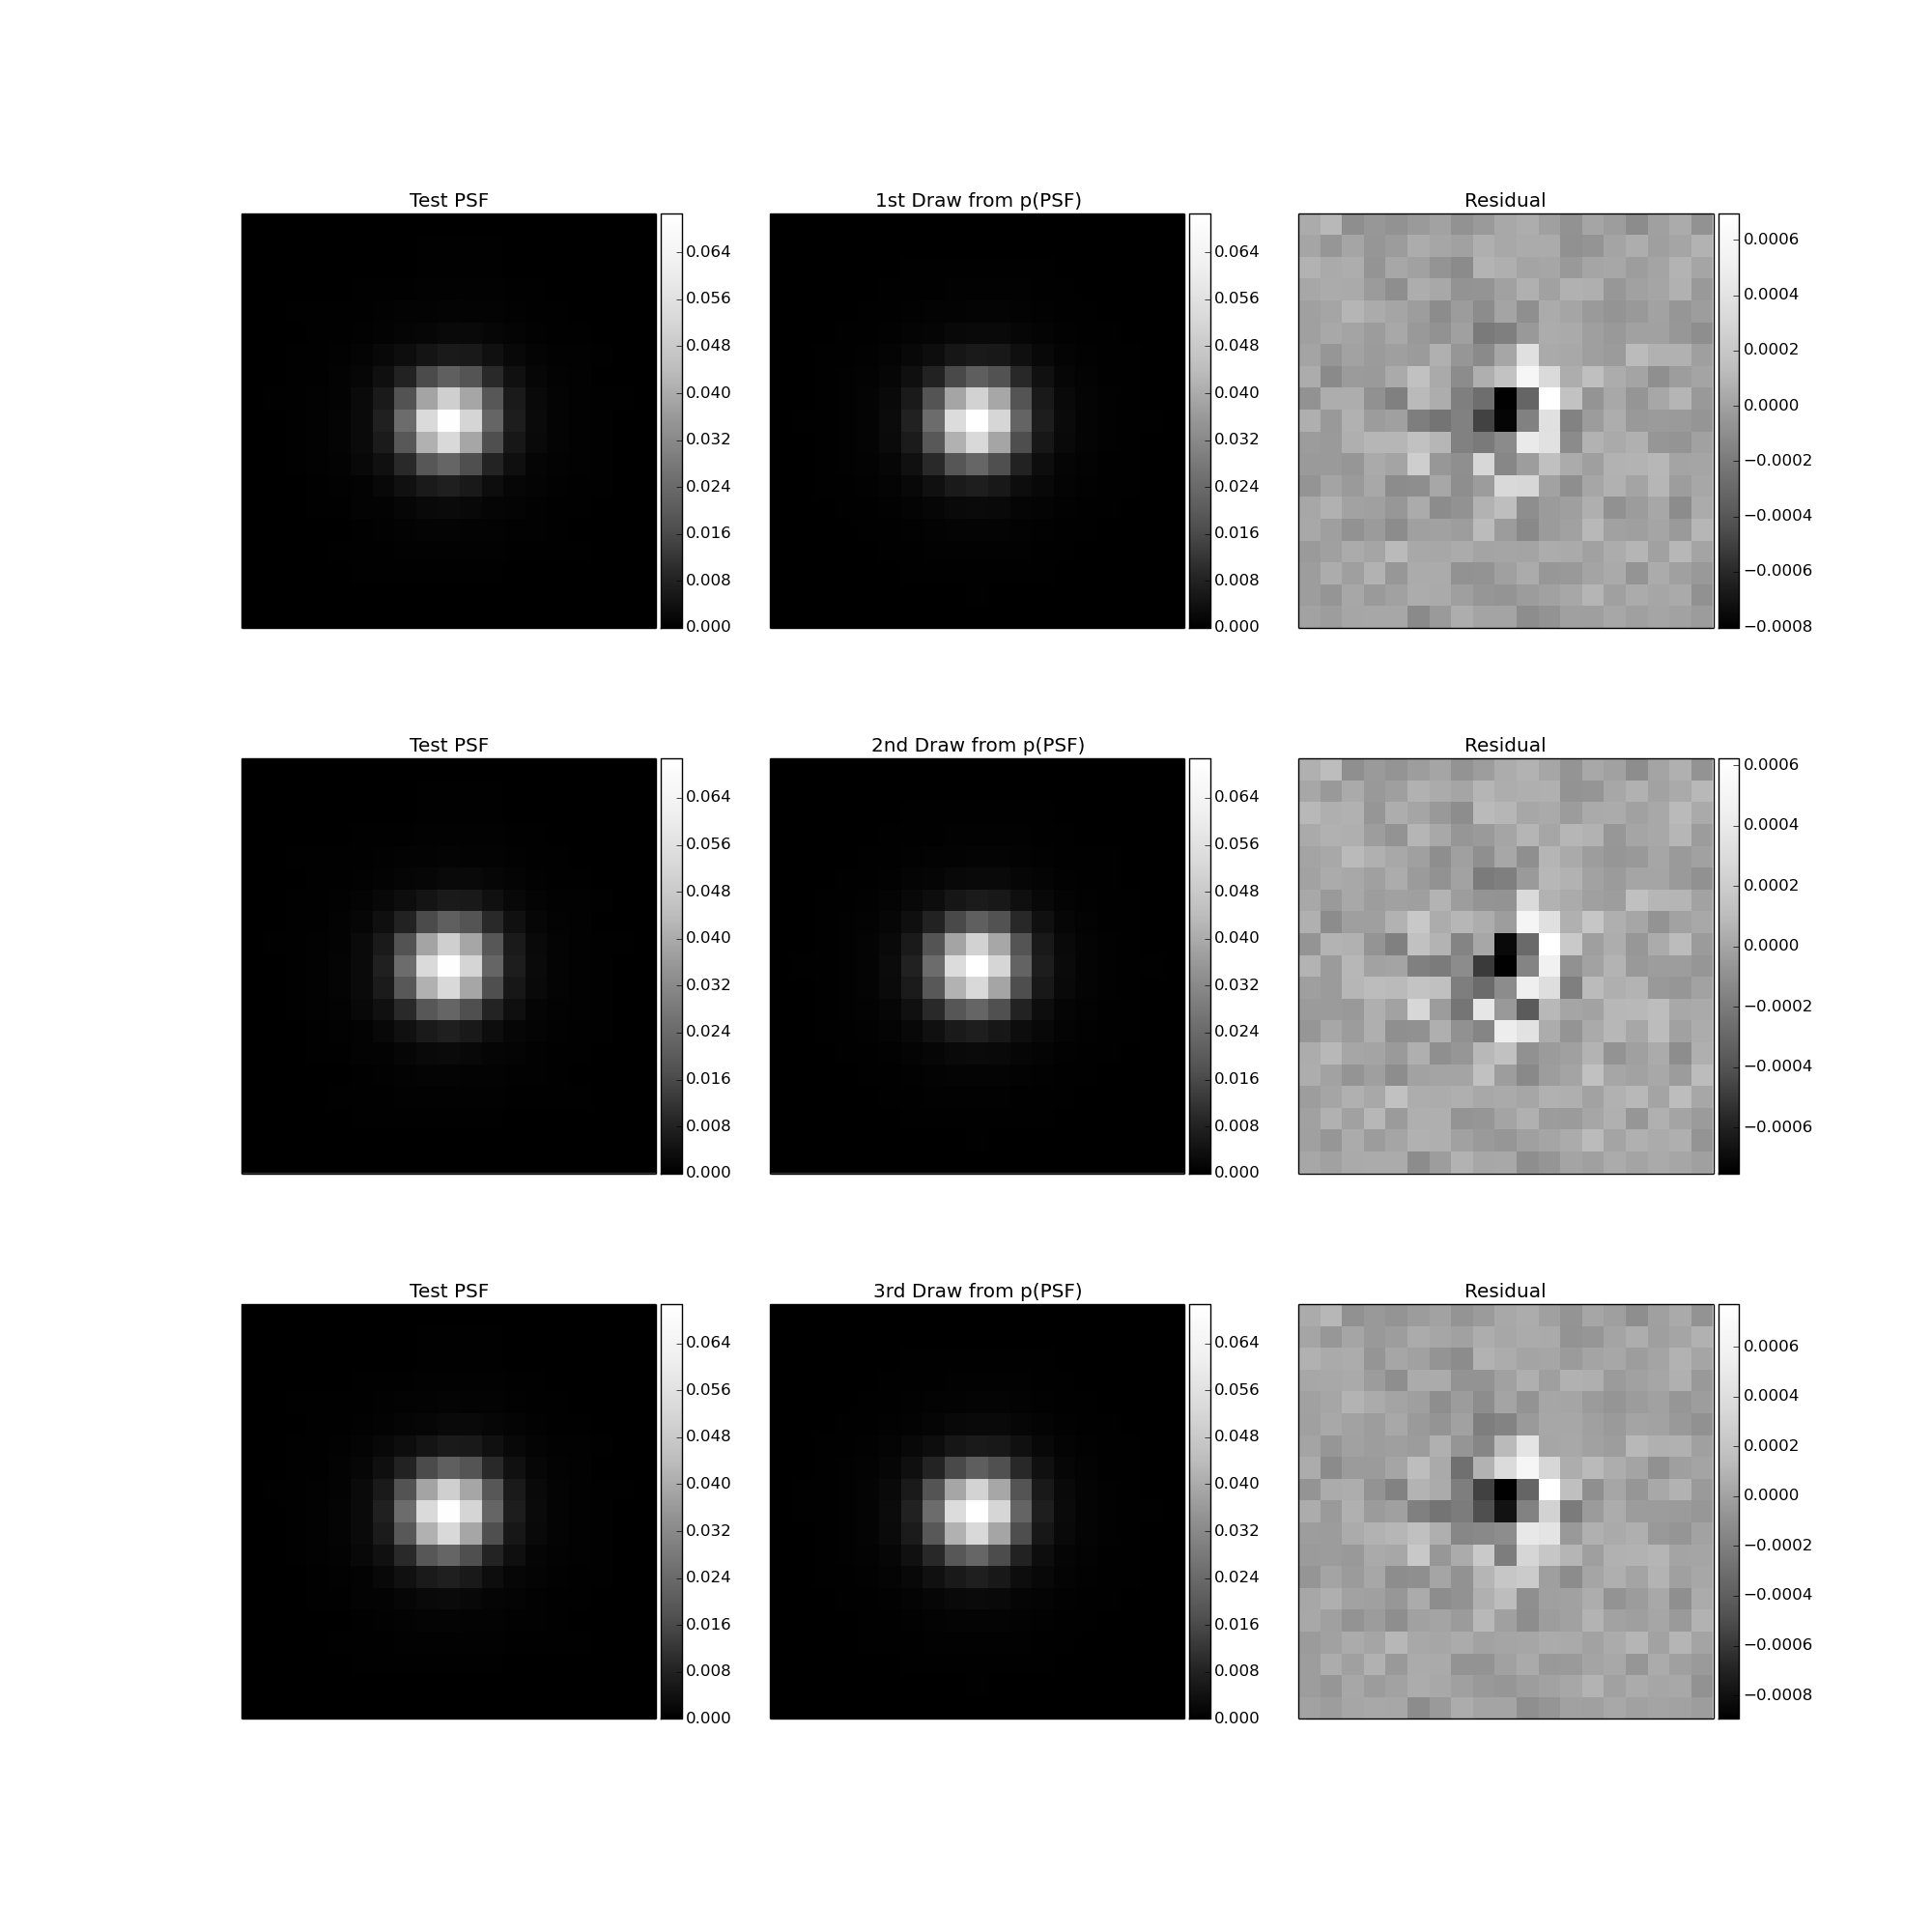
\includegraphics[width=\linewidth]{112.png}
\endminipage
\caption{Plots showing a star in the validation set
(first column), and three different draws (second column)
from our probabilistic PSF model at the
position of star, and the residuals (third column).\label{1}}
\end{figure}

\begin{figure}[!htb]

\minipage{.3\textwidth}
  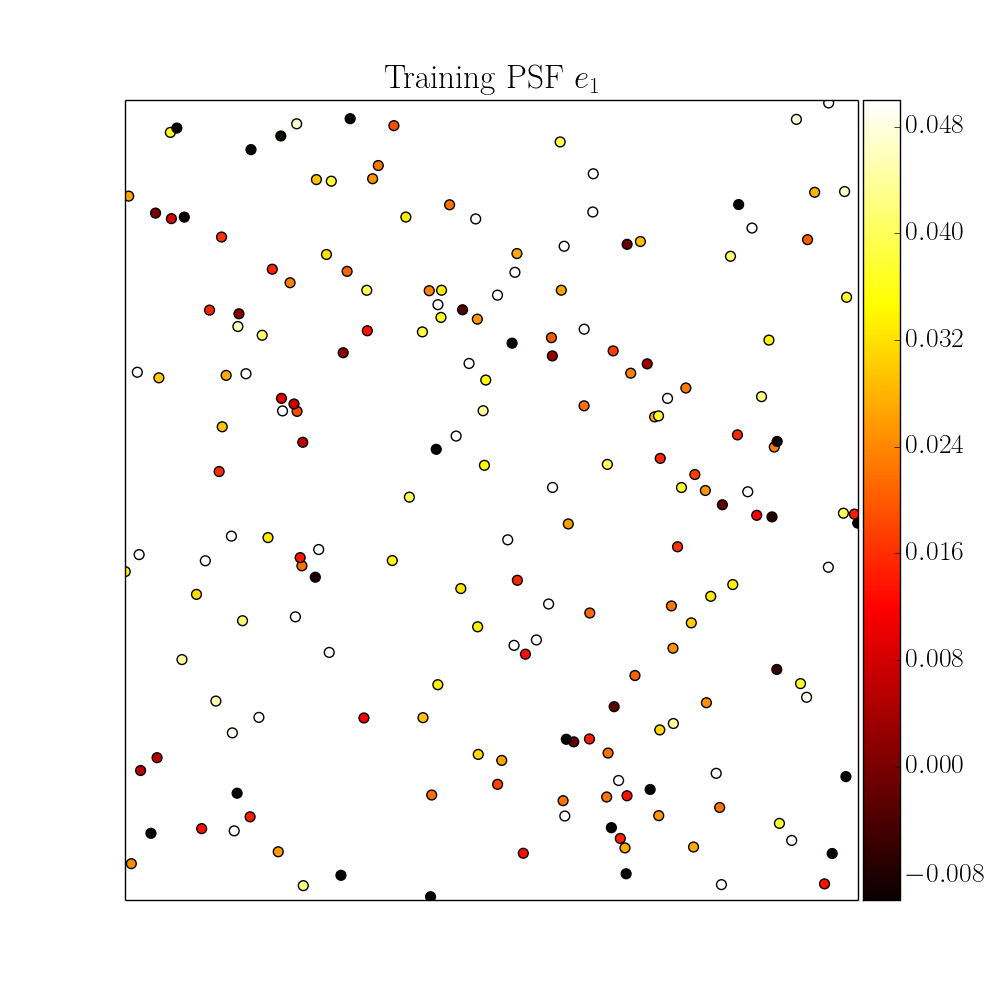
\includegraphics[width=\linewidth]{data_e1.png}
\endminipage

\minipage{1.\textwidth}
  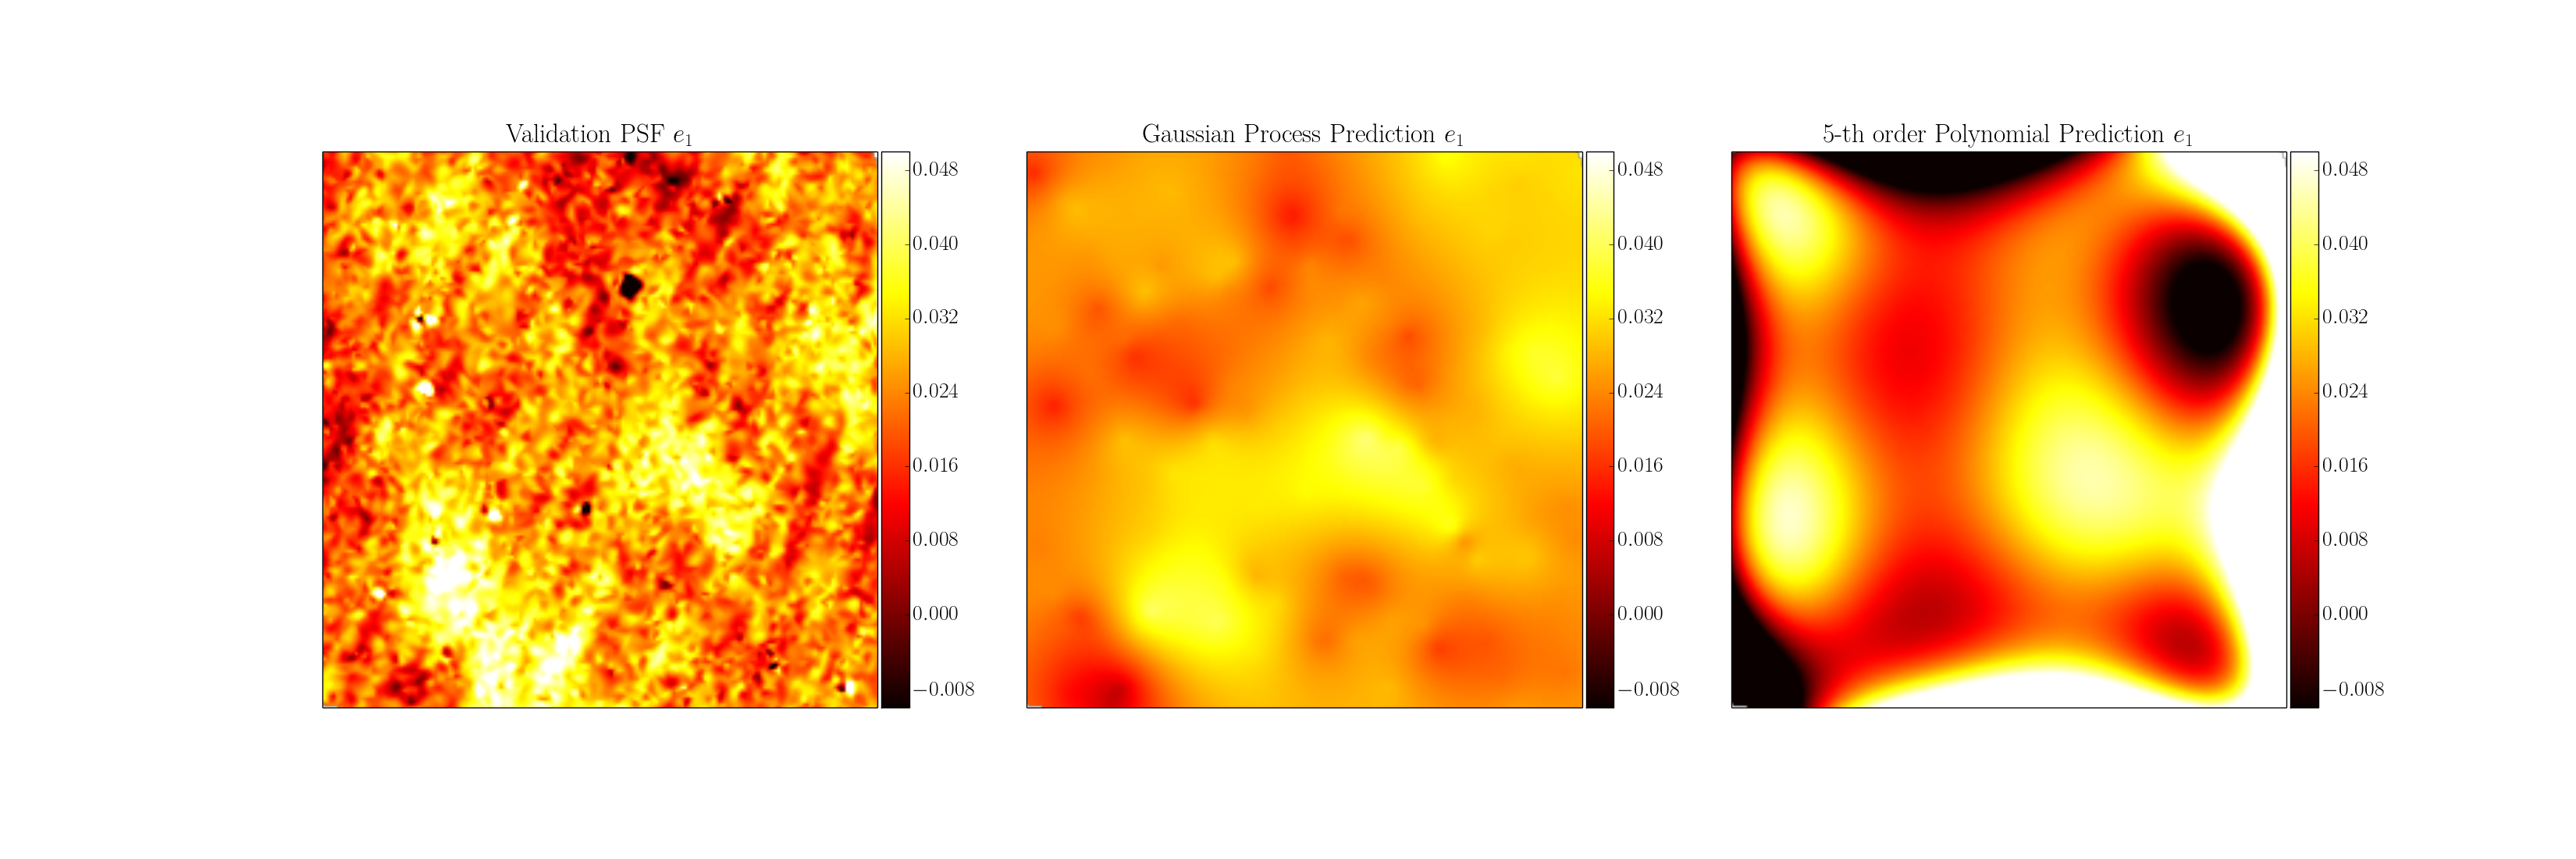
\includegraphics[width=\linewidth]{validation_e1.png}
\endminipage

\caption{Top: scatter plot showing the first components of the ellipticities
of the atmospheric PSF in LSST short exposure imaging data. 
Bottom: Map showing the underlying pattern of atmospheric PSF ellipticities (left),
mean of the posterior probability(middle), and the prediction of 5-th
order polynomial regression (right).
\label{2}}
\end{figure}

\begin{figure}[!htb]
\minipage{.8\textwidth}
  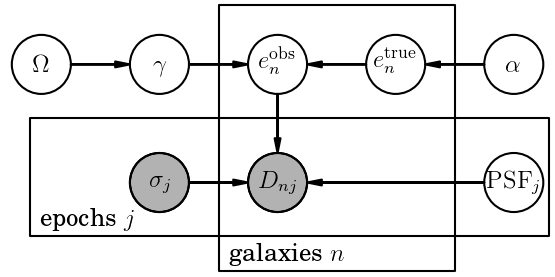
\includegraphics[width=\linewidth]{weaklensing1.png}
\endminipage
\caption{PGM showing the flow of information
from cosmological parameters $\Omega$, PSF at different
exposures $\psf_j$, and 
the underlying distribution of shape parameters 
$\alpha$, to the data at each exposure $\data_{nj}$.\label{3}}
\end{figure}

\end{document}
